\chapter{CANONICAL TRANSFORMATION}
For each problem there may be one particular choice for which all coordinates $q_i$ are cyclic. Then the conjugate momenta $p_i$ are all constant:
\begin{align*}
p_i&=\alpha_i\\
\text{Consider a situation in which }&\text{Hamiltonian is a constant of motion,
	then }\\
H&=H(\alpha_1,.......\alpha_n)\\
\text{so the Hamiltonian equations}&\text{ for $\dot{q}_i$ are }\\
\dot{q}_i&=\frac{\partial H}{\partial \alpha_i}=\omega_i\\
\text{Where $\omega_i$'s are functions of  }&\text{$\omega_i$'s only	$\therefore $ solutions are}\\
 q_i&=\omega_i t+\beta_i\\
 \text{where $\beta_i$'s are constants }&\text{of integration.}
\end{align*}
\par Since the obivious generalized coordinates suggested by the problem will
not normally be cyclic, we must have a specific proceedure for transforming from one set of variables to some other set that may be more suitable.\\\\
 In the Hameltonian formulation the momenta are also independent variable on the same level as the generalized coordinates. The similtaneous transformation of the independent coordinates and momenta $q_i,p_i$ to a new se t  $Q_i,P_i$ with (invertible) equation of transformation:
 \begin{align*}
 Q_i&=Q_i (q,p,t)\\
 P_i&=P_i (q,p,t)\\
 \text{Which define a point transfo}&\text{rmation in phase space.}
 \end{align*}
\section{Jacobian}
If $u$ and $v$ are two function of two independent variables $x$ and $y$ then the determinant $J=\left|\begin{array}{ll}\frac{\partial u}{\partial x} & \frac{\partial u}{\partial y} \\ \frac{\partial v}{\partial x} & \frac{\partial v}{\partial y}\end{array}\right|$ is called the Jacobian of $u$ and $v$ with respect to of $x$ and $y$ which is written as $\frac{\partial(u, v)}{\partial(x, y)}$ or $J\left(\frac{u, v}{x, y}\right)$\\
If $u, v$ and $w$ are three functions of three independent variables $x, y$ and $z$ then the determinant\\
$J=\left|\begin{array}{lll}\frac{\partial u}{\partial x} & \frac{\partial u}{\partial y} & \frac{\partial u}{\partial z} \\ \frac{\partial v}{\partial x} & \frac{\partial v}{\partial y} & \frac{\partial v}{\partial z} \\ \frac{\partial w}{\partial x} & \frac{\partial w}{\partial y} & \frac{\partial w}{\partial z}\end{array}\right|$
is called the Jacobian of $u, v$ and $w$ with respect to of $x, y$ and $z$
which is written as $\frac{\partial(u, v, w)}{\partial(x, y, z)}$ or $J\left(\frac{u, v, w}{x, y, z}\right)$
\subsection{Properties of Jacobian}
\begin{itemize}
	\item  If $J=\frac{\partial(u, v, w)}{\partial(x, y, z)}$ and $J^{\prime}=\frac{\partial(x, y, z)}{\partial(u, v, w)}$ then $J J^{\prime}=1$
	\item Chain rule for Jacobian if $u, v$ are functions of $r, s$ and $r, s$ functions of $x, y$ then $\frac{\partial(u, v)}{\partial(x, y)}=\frac{\partial(u, v)}{\partial(r, s)} \cdot \frac{\partial(r, s)}{\partial(x, y)}$
	\item If $u_{1}, u_{2}, u_{3}$ instead of being given explicitly in terms $x_{1}, x_{2}, x_{3}$ be connected with them with equations such as
	$$
	f_{1}\left(u_{1}, u_{2}, u_{3}, x_{1}, x_{2}, x_{3}\right)=0 f_{2}\left(u_{1}, u_{2}, u_{3}, x_{1}, x_{2}, x_{3}\right)=0 f_{3}\left(u_{1}, u_{2}, u_{3}, x_{1}, x_{2}, x_{3}\right)=0
	$$
	then $\frac{\partial\left(u_{1}, u_{2}, u_{3}\right)}{\partial\left(x_{1}, x_{2}, x_{3}\right)}=(-1)^{3} \frac{\partial\left(f_{1}, f_{2}, f_{3}\right)}{\partial\left(x_{1}, x_{2}, x_{3}\right)} / \frac{\partial\left(f_{1}, f_{2}, f_{3}\right)}{\partial\left(u_{1}, u_{2}, u_{3}\right)}$
	\\\\$\left((-1)^{3}\right.$ is for three variable system $)$
	\item  If $u_{1}, u_{2}, u_{3}$ be functions of $x_{1}, x_{2}, x_{3}$ then the necessary and sufficient condition for existence of a functional relationship of the form $f_{1}\left(u_{1}, u_{2}, u_{3}\right)=0$ is $J\left[\frac{\partial\left(u_{1}, u_{2}, u_{3}\right)}{\partial\left(x_{1}, x_{2}, x_{3}\right)}\right]=0$
\end{itemize}
\section{Canonical Transformation}
	 In Hamiltonian mechanics the transformation should be such that $Q$ and $P$ are canonical coordinates
	We would like to change variables from the set $(a,p)$ to a new set $(Q,P )$ such that:
	\begin{enumerate}
		\item  Determinent of Jacobian matrix of transformation, $\left| \frac{\partial(Q,P)}{\partial(q,p)}\right|=+1 $
		(This ensures that it is volume and orientation are preserved during transformation)
		\item  Ensures structure of Hamilton's equation is not changed, so the exist a function $K=K(Q,P,t)$ 
		such that the equation of motion of new set are	
		$$\dot{Q_i}-\frac{\partial K}{\partial P_i}\quad,\quad\dot{P_i}=\frac{\partial K}{\partial Q_i}$$
		$K$ plays role of Hamiltonian in new coordinate set and known as 'kamiltonian'	
	\end{enumerate}
\begin{note}
	The transformation considered be problem independent that is to say $(Q,P)$ must be canonical coordinates not onlu for some specific mechanical systems, but for all systems of the same number of degrees of freedom.	
\end{note}
\textbf{Hamilton's Priciple of Transformed Coordinates}\vspace{0.1cm}\\
 As $Q_i$ and $P_i$ are canonical variable they must satisfy Hamiltonians principle
\begin{equation}
\delta\int\limits_{t_1}^{t_2}(P_i\dot{Q_i}-K(Q,P,t))dt=0
\end{equation}
as of old canonical variables
\begin{equation}
\delta\int\limits_{t_1}^{t_2}(p_i\dot{q_i}-H(Q,P,t))dt=0
\end{equation}
\begin{align*}
\therefore\quad \text{ we can say}\\
\lambda (p_i\dot{q_i}-H)&=P_i\dot{Q_i}-K+\frac{\partial F}{\partial t}\\
\text{$F$ is a function }&\text{of phase space coordinates with continuous second derivatives}\\
\intertext{$\lambda$ is a constant independent of canonical coordinates and the time and it is related to scale transformation. }
\text{For }\lambda&=1\text{ we have}\\
p_i\dot{q_i}-H&=P_i\dot{Q_i}-K+\frac{dF}{dt}\\
\text{Which is simply}&\text{ called canonical transformation }
\end{align*}





\begin{note}
	A transformation of canonical coordinates for which is called extended canonical transformation
\end{note}
Canonical Transformation have following four properties
\begin{enumerate}
	\item The identity transformation is canonical.
	\item If a transformation is canonical, so is its inverse.
	\item Two successive canonical transformations (the group "product" operation) define a transformation that is also canonical.
	\item The product operation is associative.
\end{enumerate}
\section{Generating Function}
\begin{itemize}
	\item The term $\frac{df}{dt}$ in canonical transformation contributes to the variation of action integral only at the end points, and will vanish if $F$ is a function of $(q,p t)$ or $(Q,P,t)$or any mixture of the phase space coordinates since these have zero variation at the end points.
	\item Through equations of transformation and their inverses $F$ can be expressed partly in terms of the old set of variables and partly of the new.
	\item $F$ acts as a bridge between the two sets of canonical variables and is called the generating function of transformation.
\end{itemize}
There are four types of generating function:
\begin{enumerate}
	\item  $F=F_{1}\left(q_{i}, Q_{i}, t\right)$ known as $F_{1}\left(q_{i}, Q_{i}, t\right)$ is $F_{1}$ type Generating function.
	$$
	\begin{aligned}
	\left(\sum_{i} p_{i} \dot{q}_{i}-H\right)&=\left(\sum_{i} P_{i} \dot{Q}_{i}-K\right)+\frac{d F}{d t} \Rightarrow\left(\sum_{i} p_{i} \dot{q}_{i}-H\right)=\left(\sum_{i} P_{i} \dot{Q}_{i}-K\right)+\frac{d F_{1}}{d t} \\
	\Rightarrow\left(\sum_{i} p_{i} \dot{q}_{i}-H\right)&=\left(\sum_{i} P_{i} \dot{Q}_{i}-K\right)+\sum_{i} \frac{\partial F_{1}}{\partial q_{i}} \dot{q}_{i}+\sum_{i} \frac{\partial F_{1}}{\partial Q_{i}} \dot{Q}_{i}+\frac{\partial F}{\partial t}\\
	\text{	Comparing both the }&\text{coefficient of $\dot{q}_{i}$ and $\dot{Q}_{i}$}\\
	\frac{\partial F_{1}}{\partial q_{i}}=p_{i} \quad \frac{\partial F_{1}}{\partial Q_{i}}&=-P_{i}\text{ and }K=H+\frac{\partial F_{1}}{\partial t}
	\end{aligned}
	$$
	\item $F=F_{2}\left(q_{i}, P_{i}, t\right)-Q_{i} P_{i}$ known as $F_{2}\left(q_{i}, P_{i}, t\right)$ is $F_{2}$ type Generating function.\\
	$$
	\begin{aligned}
	\left(\sum_{i} p_{i} \dot{q}_{i}-H\right)&=\left(\sum_{i} P_{i} \dot{Q}_{i}-K\right)+\frac{d F}{d t} \\
	\Rightarrow\left(\sum_{i} p_{i} \dot{q}_{i}-H\right)&=\left(\sum_{i} P_{i} \dot{Q}_{i}-K\right)-\sum_{i} \dot{Q}_{i} P_{i}-\sum_{i} Q_{i} \dot{P}_{i}-\frac{d F_{2}}{d t} \\
	\Rightarrow\left(\sum_{i} p_{i} \dot{q}_{i}-H\right)&=\left(\sum_{i} P_{i} \dot{Q}_{i}-K\right)+\sum_{i} \frac{\partial F_{2}}{\partial q_{i}} \dot{q}_{i}+\sum_{i} \frac{\partial F_{2}}{\partial P_{i}} \dot{P}_{i}+\frac{\partial F_{2}}{\partial t}-\sum_{i} \dot{Q}_{i} P_{i}-\sum_{i} Q_{i} \dot{P}_{i}\\
	\text{Comparing both the }&\text{coefficient of $\dot{q}_{i}$ and $\dot{P}_{i}$}\\
	\frac{\partial F_{2}}{\partial q_{i}}=p_{i}, \ \frac{\partial F_{2}}{\partial P_{i}}&=Q_{i}\text{ and }K=H+\frac{\partial F_{2}}{\partial t}
	\end{aligned}
	$$
	\item  $F=F_{3}\left(Q_{i}, p_{i}, t\right)+q_{i} p_{i}$ known as $F_{3}\left(Q_{i}, p_{i}, t\right)$ is $F_{3}$ type Generating function.
	$$
	\begin{aligned}
	\left(\sum_{i} p_{i} \dot{q}_{i}-H\right)&=\left(\sum_{i} P_{i} \dot{Q}_{i}-K\right)+\frac{d F}{d t} \\
	\Rightarrow\left(\sum_{i} p_{i} \dot{q}_{i}-H\right)&=\left(\sum_{i} P_{i} \dot{Q}_{i}-K\right)+\frac{d F_{3}}{d t}+\sum_{i} \dot{q}_{i} p_{i}+\sum_{i} q_{i} \dot{p}_{i} \\
	\Rightarrow\left(\sum_{i} p_{i} \dot{q}_{i}-H\right)&=\left(\sum_{i} P_{i} \dot{Q}_{i}-K\right)+\sum_{i} \frac{\partial F_{3}}{\partial Q_{i}} \dot{Q}_{i}+\sum_{i} \frac{\partial F_{3}}{\partial p_{i}} \dot{p}_{i}+\frac{\partial F_{3}}{\partial t}+\sum_{i} \dot{q}_{i} p_{i}+\sum_{i} q_{i} \dot{p}_{i}\\
	\text{	Comparing both the }&\text{coefficient of $\dot{q}_{i}$ and $\dot{P}_{i}$}\\
	\frac{\partial F_{3}}{\partial Q_{i}}=-P_{i},\  \frac{\partial F_{3}}{\partial p_{i}}&=-q_{i}\text{ and }K=H+\frac{\partial F_{3}}{\partial t}
	\end{aligned}
	$$
	\item  $F=F_{4}\left(p_{i}, P_{i}, t\right)+q_{i} p_{i}-Q_{i} P_{i}$ known as $F_{3}\left(P_{i}, p_{i}, t\right)$ is $F_{3}$ type Generating function.
	$$
	\begin{aligned}
	\left(\sum_{i} p_{i} \dot{q}_{i}-H\right)&=\left(\sum_{i} P_{i} \dot{Q}_{i}-K\right)+\frac{d F}{d t} \\
	\Rightarrow\left(\sum_{i} p_{i} \dot{q}_{i}-H\right)&=\left(\sum_{i} P_{i} \dot{Q}_{i}-K\right)+\frac{d F_{4}}{d t}+\sum_{i} \dot{q}_{i} p_{i}+\sum_{i} q_{i} \dot{p}_{i}-\sum_{i} \dot{Q}_{i} P_{i}-\sum_{i} Q_{i} \dot{P}_{i}\\
	\Rightarrow\left(\sum_{i} p_{i} \dot{q}_{i}-H\right)&=\left(\sum_{i} P_{i} \dot{Q}_{i}-K\right)+\sum_{i} \frac{\partial F_{4}}{\partial P_{i}} \dot{P}_{i}+\sum_{i} \frac{\partial F_{4}}{\partial p_{i}} \dot{p}_{i}+\frac{\partial F_{4}}{\partial t}+\sum_{i} \dot{q}_ip_i+q_i\dot{p}_i-\sum_{i} \dot{Q}_iP_i-\sum_{i} Q_i\dot{P}_i\\
	\text{Comparing both }&\text{the coefficient of $\dot{p}_{i}$ and $\dot{P}_{i}$}\\
	\frac{\partial F_{4}}{\partial p_{i}}=-q_{i},\  \frac{\partial F_{4}}{\partial P_{i}}&=Q_{i} \text { and } K=H+\frac{\partial F_{4}}{\partial t}
	\end{aligned}
	$$
\end{enumerate}
	\begin{table}[H]
	\centering
	\renewcommand*{\arraystretch}{1.8}
	\begin{tabular}{|p{4.5cm}|p{5cm}|p{5.5cm}|}	
	\hline Generating Function&Generating Function Derivatives&Trivial Special Case\\
	\hline $F=F_{1}(q, Q, t)$&$p_{i}=\frac{\partial F_{1}}{\partial q_{i}} \quad P_{i}=-\frac{\partial F_{1}}{\partial Q_{i}}$&$F_{1}=q_{i} Q_{i}, \quad Q_{i}=p_{i}, \quad P_{i}=-q_{i}$\\
	\hline $F=F_{2}(q, P, t)-Q_{i} P_{i}$&$p_{i}=\frac{\partial F_{2}}{\partial q_{i}} \quad Q_{i}=\frac{\partial F_{2}}{\partial P_{i}}$&$F_{2}=q_{i} P_{i}, \quad Q_{i}=q_{i}, \quad P_{i}=p_{i}$\\
	\hline $F=F_{3}(p, Q, t)+q_{i} p_{i}$&$q_{i}=-\frac{\partial F_{3}}{\partial p_{i}} \quad P_{i}=-\frac{\partial F_{3}}{\partial Q_{i}}$&$F_{3}=p_{i} Q_{i}, \quad Q_{i}=-q_{i}, \quad P_{i}=-p_{i}$\\
	\hline $F=F_{4}(p, P, t)+q_{i} p_{i}-Q_{i} P_{i}$&$q_{i}=-\frac{\partial F_{4}}{\partial p_{i}} \quad Q_{i}=\frac{\partial F_{4}}{\partial P_{i}}$&$F_{4}=p_{i} P_{i}, \quad Q_{i}=p_{i}, \quad P_{i}=-q_{i}$\\\hline
	\end{tabular}
\end{table}
\newpage
\begin{abox}
	Practise set-1
\end{abox}
\begin{enumerate}
	\item  Let $q$ and $p$ be the canonical coordinate and momentum of a dynamical system. Which of the following transformations is canonical?
	1. $Q_{1}=\frac{1}{\sqrt{2}} q^{2}$ and $P_{1}=\frac{1}{\sqrt{2}} p^{2}$
	2. $Q_{2}=\frac{1}{\sqrt{2}}(p+q)$ and $P_{2}=\frac{1}{\sqrt{2}}(p-q)$
	{\exyear{ NET/JRF (June-2015)}}
	 \begin{tasks}(2)
		\task[\textbf{a.}]Neither 1 nor 2
		\task[\textbf{b.}]Both 1 and 2
		\task[\textbf{c.}]Only 1
		\task[\textbf{d.}] Only 2
	\end{tasks}
	\item  Let $x$ denote the position operator and $p$ the canonically conjugate momentum operator of a particle. The commutator
	$$
	\left[\frac{1}{2 m} p^{2}+\beta x^{2}, \frac{1}{m} p^{2}+\gamma x^{2}\right]
	$$
	where $\beta$ and $\gamma$ are constants, is zero if
	{\exyear{ NET-JRF (Dec-2017)}}
	 \begin{tasks}(4)
		\task[\textbf{a.}]$\gamma=\beta$
		\task[\textbf{b.}]$\gamma=2 \beta$
		\task[\textbf{c.}]$\gamma=\sqrt{2} \beta$
		\task[\textbf{d.}] $2 \gamma=\beta$
	\end{tasks}
	\item  A Hamiltonian system is described by the canonical coordinate $q$ and canonical momentum $p$. A new coordinate $Q$ is defined as $Q(t)=q(t+\tau)+p(t+\tau)$, where $t$ is the time and $\tau$ is a constant, that is, the new coordinate is a combination of the old coordinate and momentum at a shifted time. The new canonical momentum $P(t)$ can be expressed as
{\exyear{	NET/JRF (June-2017)}}
	 \begin{tasks}(2)
		\task[\textbf{a.}]$p(t+\tau)-q(t+\tau)$
		\task[\textbf{b.}]$p(t+\tau)-q(t-\tau)$
		\task[\textbf{c.}]$\frac{1}{2}[p(t-\tau)-q(t+\tau)]$
		\task[\textbf{d.}] $\frac{1}{2}[p(t+\tau)-q(t+\tau)]$
	\end{tasks}
	\item  Let $(x, p)$ be the generalized coordinate and momentum of a Hamiltonian system. If new variables $(X, P)$ are defined by $X=x^{\alpha} \sinh (\beta p)$ and $P=x^{\gamma} \cosh (\beta p)$, where $\alpha, \beta$ and $\gamma$ are constants, then the conditions for it to be a canonical transformation, are
	NET/JRF (DEC-2017)
	 \begin{tasks}(2)
		\task[\textbf{a.}]$\alpha=\frac{1}{2 \beta}(\beta+1)$ and $\gamma=\frac{1}{2 \beta}(\beta-1)$
		\task[\textbf{b.}]$\beta=\frac{1}{2 \gamma}(\alpha+1)$ and $\gamma=\frac{1}{2 \alpha}(\alpha-1)$
		\task[\textbf{c.}]$\alpha=\frac{1}{2 \beta}(\beta-1)$ and $\gamma=\frac{1}{2 \beta}(\beta+1)$
		\task[\textbf{d.}] $\beta=\frac{1}{2 \gamma}(\alpha-1)$ and $\gamma=\frac{1}{2 \alpha}(\alpha+1)$
	\end{tasks}
	\item  A canonical transformation relates the old coordinates $(q, p)$ to the new ones $(Q, P)$ by the relations $Q=q^{2}$ and $P=p / 2 q$. The corresponding time independent generating function is
	{\exyear{ 	NET/JRF (June-2014)}}
	 \begin{tasks}(4)
		\task[\textbf{a.}]$P / q^{2}$
		\task[\textbf{b.}]$q^{2} P$
		\task[\textbf{c.}]$q^{2} / P$
		\task[\textbf{d.}] $q P^{2}$ 
	\end{tasks}
	\item  A mechanical system is described by the Hamiltonian $H(q, p)=\frac{p^{2}}{2 m}+\frac{1}{2} m \omega^{2} q^{2}$. As a result of the canonical transformation generated by $F(q, Q)=-\frac{Q}{q}$, the Hamiltonian in the new coordinate $Q$ and momentum $P$ becomes
{\exyear{ 	NET/JRF (DEC-2014)}}
	 \begin{tasks}(2)
		\task[\textbf{a.}] $\frac{1}{2 m} Q^{2} P^{2}+\frac{m \omega^{2}}{2} Q^{2}$
		\task[\textbf{b.}]$\frac{1}{2 m} Q^{2} P^{2}+\frac{m \omega^{2}}{2} P^{2}$
		\task[\textbf{c.}]$\frac{1}{2 m} P^{2}+\frac{m \omega^{2}}{2} Q^{2}$
		\task[\textbf{d.}] $\frac{1}{2 m} Q^{2} P^{4}+\frac{m \omega^{2}}{2} P^{-2}$
	\end{tasks}
	\item  A canonical transformation $(q, p) \rightarrow(Q, P)$ is made through the generating function $F(q, P)=q^{2} P$ on the Hamiltonian
	$$
	H(q, p)=\frac{p^{2}}{2 \alpha q^{2}}+\frac{\beta}{4} q^{4}
	$$
	where $\alpha$ and $\beta$ are constants. The equations of motion for $(Q, P)$ are
{\exyear{ 	NET/JRF (June-2016)}}
	 \begin{tasks}(2)
		\task[\textbf{a.}] $\dot{Q}=\frac{P}{\alpha}$ and $\dot{P}=-\beta Q$
		\task[\textbf{b.}] $\dot{Q}=\frac{4 P}{\alpha}$ and $\dot{P}=\frac{-\beta Q}{2}$
		\task[\textbf{c.}]$\dot{Q}=\frac{P}{\alpha}$ and $\dot{P}=-\frac{2 P^{2}}{Q}-\beta Q$
		\task[\textbf{d.}] $\dot{Q}=\frac{2 P}{\alpha}$ and $\dot{P}=-\beta Q$
	\end{tasks}
	\item  A canonical transformation $(p, q) \rightarrow(P, Q)$ is performed on the Hamiltonian $H=\frac{p^{2}}{2 m}+\frac{1}{2} m \omega^{2} q^{2}$ via the generating function, $F=\frac{1}{2} m \omega q^{2} \cot Q$. If $Q(0)=0$, which of the following graphs shows schematically the dependence of $Q(t)$ on $t$ ?
	 \begin{tasks}(2)
		\task[\textbf{a.}]
		\begin{figure}[H]
			\centering
			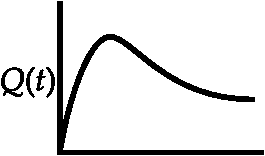
\includegraphics[height=1.5cm,width=2.5cm]{CE-01}
		\end{figure}
		\task[\textbf{b.}]	\begin{figure}[H]
			\centering
			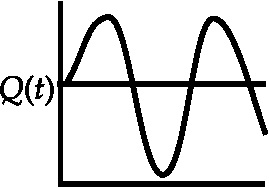
\includegraphics[height=1.5cm,width=2.5cm]{cE-02}
		\end{figure}
		\task[\textbf{c.}]
		\begin{figure}[H]
			\centering
			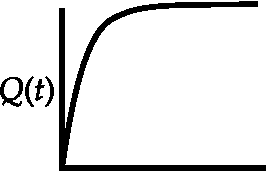
\includegraphics[height=1.5cm,width=2.5cm]{CN-03}
		\end{figure}
		\task[\textbf{d.}] \begin{figure}[H]
			\centering
			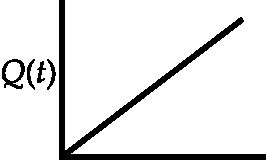
\includegraphics[height=1.5cm,width=2.5cm]{CN-04}
		\end{figure}
	\end{tasks}
	\item  The generator of the infinitesimal canonical transformation $q \rightarrow q^{\prime}=(1+\epsilon) q$ and $p \rightarrow p^{\prime}=(1-\in) p$ is
{\exyear{ 	NET/JRF (DEC-2019)}}
	 \begin{tasks}(4)
		\task[\textbf{a.}] $q+p$
		\task[\textbf{b.}]$q p$
		\task[\textbf{c.}]$\frac{1}{2}\left(q^{2}-p^{2}\right)$
		\task[\textbf{d.}] $\frac{1}{2}\left(q^{2}+p^{2}\right)$
	\end{tasks}
	 \colorlet{ocre1}{ocre!70!}
	\colorlet{ocrel}{ocre!30!}
	\setlength\arrayrulewidth{1pt}
	\begin{table}[H]
		\centering
		\arrayrulecolor{ocre}
		\begin{tabular}{|p{1.5cm}|p{1.5cm}||p{1.5cm}|p{1.5cm}|}
			\hline
			\multicolumn{4}{|c|}{\textbf{Answer key}}\\\hline\hline
			\rowcolor{ocrel}Q.No.&Answer&Q.No.&Answer\\\hline
			1&\textbf{d} &2&\textbf{b}\\\hline 
			3&\textbf{d} &4&\textbf{c} \\\hline
			5&\textbf{b} &6&\textbf{d} \\\hline
			7&\textbf{b}&8&\textbf{d}\\\hline
			9&\textbf{b}&10&\textbf{}\\\hline
			11&\textbf{} &12&\textbf{}\\\hline
			13&\textbf{}&14&\textbf{}\\\hline
			15&\textbf{}& &\\\hline
			
		\end{tabular}
	\end{table}
\end{enumerate}
\newpage
\begin{abox}
	Practise set-2
\end{abox}
\begin{enumerate}
	\item  Let $p$ be the momentum conjugate to the generalized coordinate $q$. If the transformation
	$$
	\begin{aligned}
	&Q=\sqrt{2} q^{m} \cos p \\
	&P=\sqrt{2} q^{m} \sin p
	\end{aligned}
	$$
	is canonical, then $m=$-----------
{\exyear{	GATE- 2020}}
	\item  Let $(p, q)$ and $(P, Q)$ be two pairs of canonical variables. The transformation
	$$
	Q=q^{\alpha} \cos (\beta p), P=q^{\alpha} \sin (\beta p)
	$$
	is canonical for
{\exyear{ 	GATE- 2011}}
	 \begin{tasks}(4)
		\task[\textbf{a.}]$\alpha=2, \beta=\frac{1}{2}$
		\task[\textbf{b.}]$\alpha=2, \beta=2$
		\task[\textbf{c.}]$\alpha=1, \beta=1$
		\task[\textbf{d.}] $\alpha=\frac{1}{2}, \beta=2$
	\end{tasks}
	\item  Given that the linear transformation of a generalized coordinate $q$ and the corresponding momentum $p, Q=q+4 a p, P=q+2 p$ is canonical, the value of the constant $a$ is -------------
	{\exyear{ 	GATE- 2014}}
\item  For the transformation
$$
Q=\sqrt{2 q} e^{-1+2 \alpha} \cos p, P=\sqrt{2 q} e^{-\alpha-1} \sin p
$$
(where $\alpha$ is a constant) to be canonical, the value of $\alpha$ is-------
{\exyear{ GATE - 2018}}
	\item  Consider a transformation from one set of generalized coordinate and momentum $(q, p)$ to another set $(Q, P)$ denoted by,
	$$
	Q=p q^{s} ; \quad P=q^{r}
	$$
	where $s$ and $r$ are constants. The transformation is canonical if
{\exyear{ 	GATE - 2019}}
	 \begin{tasks}(2)
		\task[\textbf{a.}]$s=0$ and $r=1$
		\task[\textbf{b.}]$s=2$ and $r=-1$
		\task[\textbf{c.}] $s=0$ and $r=-1$
		\task[\textbf{d.}] $s=2$ and $r=1$
	\end{tasks}
	\item  If the coordinate $q$ and the momentum $p$ form a canonical pair $(q, p)$, which one of the sets given below also forms a canonical?
{\exyear{ 	JEST-2012}}
	 \begin{tasks}(4)
		\task[\textbf{a.}]$(q,-p)$
		\task[\textbf{b.}]$\left(q^{2}, p^{2}\right)$
		\task[\textbf{c.}]$(p,-q)$
		\task[\textbf{d.}] $\left(q^{2},-p^{2}\right)$
	\end{tasks}
	\item  $\left(Q_{1}, Q_{2}, P_{1}, P_{2}\right)$ and $\left(q_{1}, q_{2}, p_{1}, p_{2}\right)$ are two sets of canonical coordinates, where $Q_{i}$ and $q_{i}$ are the coordinates and $P_{i}$ and $p_{i}$ are the corresponding conjugate momenta. If $P_{1}=q_{2}$ and $P_{2}=p_{1}$, then which of the following relations is true?
	{\exyear{ JEST-2017}}
	 \begin{tasks}(2)
		\task[\textbf{a.}]$Q_{1}=q_{1}, Q_{2}=p_{2}$
		\task[\textbf{b.}]$Q_{1}=p_{2}, Q_{2}=q_{1}$
		\task[\textbf{c.}]$Q_{1}=-p_{2}, Q_{2}=q_{1}$
		\task[\textbf{d.}] $Q_{1}=q_{1}, Q_{2}=-p_{2}$
	\end{tasks}
	\item  If $(q, p)$ is a canonically conjugate pair, which of the following is not a canonically conjugate pair?
{\exyear{ 	JEST-2018}}
	 \begin{tasks}(1)
		\task[\textbf{a.}] $\left(q^{2}, \frac{p q^{-1}}{2}\right)$
		\task[\textbf{b.}]$\left(p^{2},-\frac{q p^{-1}}{2}\right)$
		\task[\textbf{c.}] $\left(p q^{-1},-q^{2}\right)$
		\task[\textbf{d.}] $\left(f(p)-\frac{q}{f^{\prime}(p)}\right)$ where $f^{\prime}(p)$ is the derivative of $f(p)$ with respect to $p$.
	\end{tasks}
	\item  Consider the following transformation of the phase space coordinates $(q, p) \rightarrow(Q, P)$
	$$
	Q=q^{a} \cos b p \quad P=q^{a} \sin b p
	$$
	For what values of $a$ and $b$ will the transformation be canonical?
{\exyear{ 	JEST-2019}}
	 \begin{tasks}(4)
		\task[\textbf{a.}]1,1
		\task[\textbf{b.}] $\frac{1}{2}, \frac{1}{2}$
		\task[\textbf{c.}]$2, \frac{1}{2}$
		\task[\textbf{d.}] $\frac{1}{2}, 2$
	\end{tasks}
	\item  The Hamiltonian of a classical particle is given by $H(p, q)=\frac{p^{2}}{2 m}+\frac{k q^{2}}{2}$. Given $F(p, q, t)=\ln (p+i m \omega q)-i \alpha \omega t$ is a constant of motion (where $\left.\omega=\sqrt{\frac{k}{m}}\right)$. What is the value of $\alpha$ ?
{\exyear{ 	JEST-2020}}
	 \begin{tasks}(4)
		\task[\textbf{a.}]$2 \pi$
		\task[\textbf{b.}]0
		\task[\textbf{c.}]1
		\task[\textbf{d.}]  $\pi$
	\end{tasks}
\end{enumerate}
 \colorlet{ocre1}{ocre!70!}
\colorlet{ocrel}{ocre!30!}
\setlength\arrayrulewidth{1pt}
\begin{table}[H]
	\centering
	\arrayrulecolor{ocre}
	\begin{tabular}{|p{1.5cm}|p{1.5cm}||p{1.5cm}|p{1.5cm}|}
		\hline
		\multicolumn{4}{|c|}{\textbf{Answer key}}\\\hline\hline
		\rowcolor{ocrel}Q.No.&Answer&Q.No.&Answer\\\hline
		1&\textbf{0.5} &2&\textbf{d}\\\hline 
		3&\textbf{0.25} &4&\textbf{2} \\\hline
		5&\textbf{b} &6&\textbf{c} \\\hline
		7&\textbf{c}&8&\textbf{c}\\\hline
		9&\textbf{d}&10&\textbf{c}\\\hline
		11&\textbf{} &12&\textbf{}\\\hline
		13&\textbf{}&14&\textbf{}\\\hline
		15&\textbf{}& &\\\hline
		
	\end{tabular}
\end{table}
\newpage
\begin{abox}
	Practise set-3
\end{abox}
\begin{enumerate}
	\item A mechanical system is described by the Hamiltonian $H(q, p)=\frac{p^{2}}{2 m}-\frac{1}{2} m \omega^{2} q^{2}$. As a result of the canonical transformation generated by $F(q, Q)=-\frac{Q}{q}$, the Hamiltonian in the new coordinate $Q$ and momentum $P$.
	\begin{answer}
		\begin{align*}
		H&=\frac{p^{2}}{2 m}+\frac{1}{2} m \omega^{2} q^{2}, \quad F=F_{1}(q, Q)=-\frac{Q}{q}\\
		\Rightarrow \frac{\partial F_{1}}{\partial q}&=p \Rightarrow \frac{Q}{q^{2}}=p\\
		\Rightarrow \frac{\partial F_{1}}{\partial Q}&=-P \Rightarrow-\frac{1}{q}=-P \Rightarrow q=\frac{1}{P}
		\intertext{From equation (a) and (b) $\Rightarrow p=Q P^{2}\quad 
			\because q=\frac{1}{P}
			$}
		H&=\frac{p^{2}}{2 m}-\frac{1}{2} m \omega^{2} q^{2}=\frac{Q^{2} P^{4}}{2 m}-\frac{1}{2} m \omega^{2}\left(\frac{1}{P^{2}}\right)=\frac{1}{2 m} Q^{2} P^{4}-\frac{1}{2} m \omega^{2} P^{-2}
		\end{align*}
	\end{answer}
	\item The transformation equations between two sets of coordinate are
	$$
	\begin{aligned}
	&Q=\log \left(1+q^{1 / 2} \cos p\right) \\
	&P=2\left(1+q^{1 / 2} \cos p\right) q^{1 / 2} \sin p
	\end{aligned}
	$$
	(a) Show that $Q, P$ are canonical transform to $q, p$.\\
	(b) Show that the function that generates this transformation is $F_{3}=-\left(e^{Q}-1\right)^{2} \tan p$
	\begin{answer}
		\begin{align*}
		Q&=\log \left(1+q^{\frac{1}{2}} \cos p\right)\\
		P&=2\left(1+q^{\frac{1}{2}} \cos p\right) q^{\frac{1}{2}} \sin p \Rightarrow 2 q^{\frac{1}{2}} \sin p+q \sin 2 p\\
	\text{	(a) For canonical }&\text{transformation:}
		\frac{\partial Q}{\partial q} \cdot \frac{\partial P}{\partial p}-\frac{\partial Q}{\partial p} \cdot \frac{\partial P}{\partial q}=1\\
		\Rightarrow \frac{\partial Q}{\partial q}&=\frac{1}{\left(1+q^{\frac{1}{2}} \cos p\right)} \times \frac{1}{2} q^{-\frac{1}{2}} \cos p, \frac{\partial Q}{\partial p}=\frac{q^{\frac{1}{2}}(-\sin p)}{\left(1+q^{\frac{1}{2}} \cos p\right)}\\
		\frac{\partial P}{\partial p}&=2 q^{\frac{1}{2}} \cos p+2 q \cos 2 p, \frac{\partial P}{\partial q}=2 \times \frac{1}{2} q^{-\frac{1}{2}} \sin p+\sin 2 p\\
		\Rightarrow &\frac{\cos p}{2\left(1+q^{\frac{1}{2}} \cos p\right) q^{\frac{1}{2}}} \cdot 2\left(q^{\frac{1}{2}} \cos p+q \cos 2 p\right)\\&-\frac{\left(-q^{\frac{1}{2}} \sin p\right)}{\left(1+q^{\frac{1}{2}} \cos p\right)} \times\left(q^{-\frac{1}{2}} \sin p+\sin 2 p\right)=1\\
		\text { (b) } F_{3}&=F_{3}(p, Q, t)\\
		\frac{\partial F_{3}}{\partial p}&=-q, \quad \frac{\partial F_{3}}{\partial Q}=-P\\
		Q&=\log \left(1+q^{1 / 2} \cos p\right) \Rightarrow e^{Q}=1+q^{1 / 2} \cos p\\
		\frac{e^{Q}-1}{\cos p}&=q^{1 / 2} \Rightarrow q=\left(\frac{e^{Q}-1}{\cos p}\right)^{2}\\
		P&=2\left(1+q^{1 / 2} \cos p\right) q^{1 / 2} \sin p \Rightarrow P=2 e^{Q} q^{1 / 2} \sin p \Rightarrow 2 e^{Q}\left(e^{Q}-1\right) \tan p\\
		\frac{\partial F_{3}}{\partial p}&=-q=-\frac{\left(e^{Q}-1\right)^{2}}{\cos ^{2} p} \Rightarrow F_{3}=-\int\left(e^{Q}-1\right)^{2} \sec ^{2} p d p\\
		F_{3}&=-\left(e^{Q}-1\right)^{2} \tan p+f_{1}(Q)........(A)\\
		\frac{\partial F_{3}}{\partial Q}&=-P=-2\left(e^{2 Q}-e^{Q}\right) \tan p......(B)\\
		\text { Equating A }&\text{ and B}\\
		f_{1}(Q)&=0, \quad f_{2}(p)=-\tan p\\
		\text { So } F_{3}&=-\left(e^{Q}-1\right)^{2} \tan p
		\end{align*}
	\end{answer}
	\item Prove that the transformation is canonical.\\
	(i) $Q_{1}=q_{1}, P_{1}=p_{1}-2 p_{2}$,\\
	(ii) $Q_{2}=p_{2} P_{2}=-2 q_{1}-q_{2}$
	\begin{answer}
		\begin{align*}
		&\frac{\partial Q_{1}}{\partial q_{1}} \frac{\partial P_{1}}{\partial p_{1}}-\frac{\partial Q_{1}}{\partial p_{1}} \frac{\partial P_{1}}{\partial q_{1}}+\frac{\partial Q_{1}}{\partial q_{2}} \frac{\partial P_{1}}{\partial p_{2}}-\frac{\partial Q_{1}}{\partial p_{2}} \frac{\partial P_{1}}{\partial q_{2}}=1 \times 1-0=1\\
		&\text{and }
		\frac{\partial Q_{1}}{\partial q_{1}} \frac{\partial P_{1}}{\partial p_{1}}-\frac{\partial Q_{1}}{\partial p_{1}} \frac{\partial P_{1}}{\partial q_{1}}+\frac{\partial Q_{2}}{\partial q_{2}} \frac{\partial P_{2}}{\partial p_{2}}-\frac{\partial Q}{\partial p_{2}} \frac{\partial P_{2}}{\partial q_{2}}=0-(-1)=1
		\end{align*}
	\end{answer}
	\item The Hamiltonian of harmonic oscillator is given by $H=\frac{1}{2 m}\left(p^{2}+m^{2} \omega^{2} q^{2}\right)$
\begin{tasks}(1)
	\task[\textbf{a.}]If generating function is defined as $F_{1}=\frac{m \omega q^{2}}{2} \cot Q$ then find canonical transformation.
	From the use of canonical transformation $H=\frac{1}{2 m}\left(p^{2}+m^{2} \omega^{2} q^{2}\right)$
	\task[\textbf{b.}]Find new Hamiltonian $K(Q, P, t)$
	\task[\textbf{c.}] Plot $Q$ vs $t$
	\task[\textbf{d.}]  Plot $P$ vs $t$
	\task[\textbf{e.}]Plot phase space between $P$ and $Q$
\end{tasks} 
\begin{answer}
	\begin{align*}
	\text { (a) } F_{1}&=\frac{m \omega q^{2}}{2} \cot Q, \frac{\partial F_{1}}{\partial q}=p, \frac{\partial F_{1}}{\partial Q}=-P\\
	m \omega q \cdot \cot Q&=p,-\frac{m \omega q^{2}}{2} \operatorname{cosec}{ }^{2} Q=-P\\
	q^{2}&=\frac{2 P}{m \omega} \frac{1}{\operatorname{cosec}^{2} Q}\\
	q&=\sqrt{\frac{2 P}{m \omega}} \sin Q, p=m \omega \sqrt{\frac{2 P}{m \omega}} \cot Q \sin Q\\
	p&=\sqrt{2 m P \omega} \cos Q\\
\text{	(b)}\quad
	H&=\frac{p^{2}}{2 m}+\frac{1}{2} m \omega^{2} q^{2}\\
	K&=H+\frac{\partial F_{1}}{\partial t} \Rightarrow \frac{\partial F_{1}}{\partial t}=0, K=H=\frac{1}{2 m}(\sqrt{2 P m \omega} \cos Q)^{2}+\frac{1}{2} m \omega^{2}\left(\sqrt{\frac{2 P}{m \omega}}\right)^{2} \sin ^{2} Q\\
	K&=\omega P\\
\text{	(c)}\quad
	\frac{\partial K}{\partial Q}&=-\dot{P} \Rightarrow \dot{P}=0, \frac{d P}{d t}=0, P=c\\
	\frac{\partial K}{\partial P}&=\dot{Q}=\omega, Q=\omega t+\alpha \text { where } \alpha \text { is constant, can be find with initial condition }
	\end{align*}
	\begin{figure}[H]
		\centering
		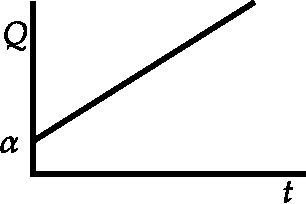
\includegraphics[height=2cm,width=3cm]{CT-03}
	\end{figure}
(d)	\begin{figure}[H]
	\centering
	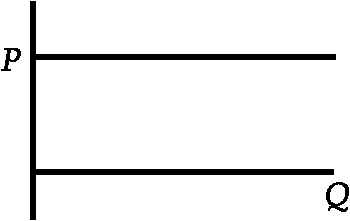
\includegraphics[height=2cm,width=3cm]{CT-02}
\end{figure}
$\hspace{2.5cm}$where $P=\frac{E}{\omega}$\\
(e)
	\begin{figure}[H]
	\centering
	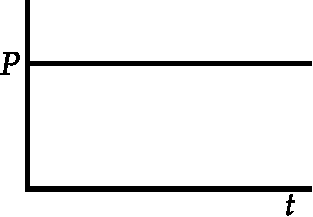
\includegraphics[height=2cm,width=3cm]{CT-01}
\end{figure}
\end{answer}
	\item If generating function is given by $F(q, P)=q^{2} P$ and Hamiltonian of the system is given by $H(q, p)=\frac{p^{2}}{2 \alpha q^{2}}+\frac{\beta q^{4}}{4}$ where $\alpha$ and $\beta$ are constants, then find the equation of motion in term of $Q, P$.
	\begin{answer}
		\begin{align*}
		F_{2}&=q^{2} P\\
		\frac{\partial F_{2}}{\partial q}&=2 q P=p, \frac{\partial F_{2}}{\partial P}=q^{2}=Q, q=\sqrt{Q}, p=2 \sqrt{Q} P\\
		K&=\frac{p^{2}}{2 \alpha q^{2}}+\frac{\beta \cdot q^{4}}{4}=\frac{4 Q P^{2}}{2 \alpha Q}+\frac{\beta Q^{2}}{4} \Rightarrow K=\frac{2 P^{2}}{\alpha}+\frac{\beta Q^{2}}{4}\\
	\frac{\partial K}{\partial P}&=\dot{Q} \Rightarrow \frac{4 P}{\alpha}=\dot{Q} \\
		\frac{\partial K}{\partial Q}&=-\dot{P} \Rightarrow \frac{\beta Q}{2}=-\dot{P}
		\end{align*}
	\end{answer}
	\item If Lagrangian of the system is given by $L=\frac{1}{2} m \dot{x}^{2}+m\left(\dot{y}^{2}+\dot{z}^{2}\right)-\frac{1}{2} k x^{2}-\frac{1}{2} k(y+z)^{2}$
	 \begin{tasks}(2)
		\task[\textbf{a.}]Write down Hamiltonian of system.
		\task[\textbf{b.}]If $L_{z}=x p_{y}-y p_{x}$, find $\frac{d L_{z}}{d t}$
		\task[\textbf{c.}]If $L_{x}=y p_{z}-z p_{y}$, find $\frac{d L_{x}}{d t}$
		\task[\textbf{d.}] If $L_{y}=z p_{x}-x p_{z}$, find $\frac{d L_{y}}{d t}$
		\task[\textbf{e.}] Find $\frac{d p_{x}}{d t}$ and $\frac{d p_{y}}{d t}$
	\end{tasks}
\begin{answer}
	\begin{align*}
	\text { (a) } \quad L&=\frac{1}{2} m \dot{x}^{2}+m\left(\dot{y}^{2}+\dot{z}^{2}\right)-\frac{1}{2} k x^{2}-\frac{1}{2} k(y+z)^{2}\\
	H&=\frac{p_{x}^{2}}{2 m}+\frac{p_{y}^{2}}{4 m}+\frac{p_{z}^{2}}{4 m}+\frac{1}{2} k x^{2}+\frac{1}{2} k(y+z)^{2}\\
	\text { (b) } \quad L_{z}&=x p_{y}-y p_{x}\\
	\frac{d L_{z}}{d t}&=\left[L_{z} H\right]+\frac{\partial L_{z}}{\partial t}, \frac{\partial L_{z}}{\partial t}=0\\
	&{\left[L_{z}, H\right]=\left[x p_{y}-y p_{x}, H\right]=x\left[p_{y}, H\right]+[x, H] p_{y}-y\left[p_{x}, H\right]-[y, H] p_{x}} \\
	&=x\left[p_{y}, \frac{1}{2} k(y+z)^{2}\right]+\left[x, \frac{p_{x}^{2}}{2 m}\right] p_{y}-y\left[p_{x}, \frac{1}{2} k x^{2}\right]-\left[y, \frac{p_{y}^{2}}{4 m}\right] p_{x} \\
	&=x(-k(y+z))+\frac{p_{x} p_{y}}{m}+k y x-\frac{p_{x} p_{y}}{2 m}\\
	\left[L_{z}, H\right]&=\frac{p_{y} p_{x}}{2 m}-k x z, \frac{d L_{z}}{d t}=\frac{p_{x} p_{y}}{2 m}-k x z\\
	\text{(c)}\quad &{\left[L_{x}, H\right]=\left[y p_{z}-z p_{y}, H\right]=\left[y p_{z}, H\right]-\left[z p_{y}, H\right]} \\
	&=[y, H] p_{z}+y\left[p_{z}, H\right]-[z, H] p_{y}-z\left[p_{y}, H\right] \\
	&=\left[y, \frac{p_{y}^{2}}{4 m}\right] p_{z}+y\left[p_{z}, \frac{1}{2} k(y+z)^{2}\right]-\left[z, \frac{p_{z}^{2}}{4 m}\right] p_{y}-z\left[p_{y}, \frac{1}{2} k(y+z)^{2}\right] \\
	&=\frac{p_{y}}{2 m} p_{z}+y[-k(y+z)]-\frac{p_{z}}{2 m} p_{y}+k z(y+z)=-k y^{2}-k z y+k z y+k z^{2}\\
	\left[L_{x}, H\right]&=k\left[z^{2}-y^{2}\right], \frac{d L_{x}}{d t}=k\left[z^{2}-y^{2}\right]\\
\text{	(d)}\quad 
	\frac{d L_{y}}{d t}&=-\frac{p_{x} p_{z}}{2 m}+k x y\\
\text{	(e)}\quad 
	\frac{\partial H}{\partial x}&=-\dot{p}_{x}, k x=-\dot{p}_{x}=\frac{-d p_{x}}{d t} \Rightarrow \frac{d p_{x}}{d t}=-k x\\
	\frac{\partial H}{\partial y}&=-\dot{p}_{y}, \frac{2 k}{2}(y+z)=-\dot{p}_{y}, \frac{d p_{y}}{d t}=-k(y+z)
	\end{align*}
\end{answer}
\end{enumerate}